\section{Experiments}
\label{sec:experiments}
Every \method{} experiment was run on a single NVIDIA A100-40GB of a DGX A100 server. All code for generation, experimentation, evaluation, and ablation studies {\modified{}is} available at \codeurl.
The images for remaining methods used in the quantitative comparison (Sec~\ref{sec:expsota}) and user study (Sec~\ref{sec:userstudy}) are taken from the PieBench experimentation files \cite{ju2023direct}. The images for the qualitative comparison (Fig.~\ref{fig:method_comparison} and Sec~\ref{sec:expsota}) corresponding to \nulltext{}, \negative{}, and \negprox{} are taken from \cite{han2023proximal}; the rest were generated with the source code of \cite{ju2023direct}, modifying hyperparameters until the best result was achieved.

As discussed in \cite{mokady2023null,han2023proximal}, all compared methods and diffusion models in general \cite{ho2021classifier} are sensitive to hyperparameters, including {\modified{}\method{}}. Nevertheless, for fairness of comparison, all \method{} results in Tables \ref{tab:ablation_piebench}, \ref{tab:comparison_piebench}, and \ref{tab:user_study} are obtained with the same hyperparameters: 50 DDIM steps, CFG scale of 7.5, local blend in the first 40 steps, cross-attention replacement in the first 5 steps, a 200 self-attention guidance scale, and 2.0 cross-attention reweighting, similar to \directinversion{} \cite{ju2023direct} configuration.


Every method uses $512 \times 512$ images and Stable Diffusion 1.4 as base diffusion model except \pnplong{}, {\modified{}which} uses 1.5. The images in Fig.~\ref{fig:teaser} are $768 \times 768$ images generated using Stable Diffusion 2.1 as the backbone of \method{}.

  
 \setlength{\tabcolsep}{1pt}

  \begin{figure*}[h]
    \footnotesize
    \small
    \centering
    \begin{tabular}{ccccccc}
      \hline

      \multirow{2}{*}{Input} &  (i) & (ii) & (iii) & (iv) & (v) & (vi) \\
      &  CA guidance &  $\vz_t$  guidance & SA replace.&  SA guidance &   (iv)+CA replace. &  (v) + LB \\
      \hline
      \multicolumn{7}{c}{``\textit{a girl with blonde hair \textcolor{RoyalBlue}{\textbf{and a fluffy rainbow hat}} smiling}"} \\
      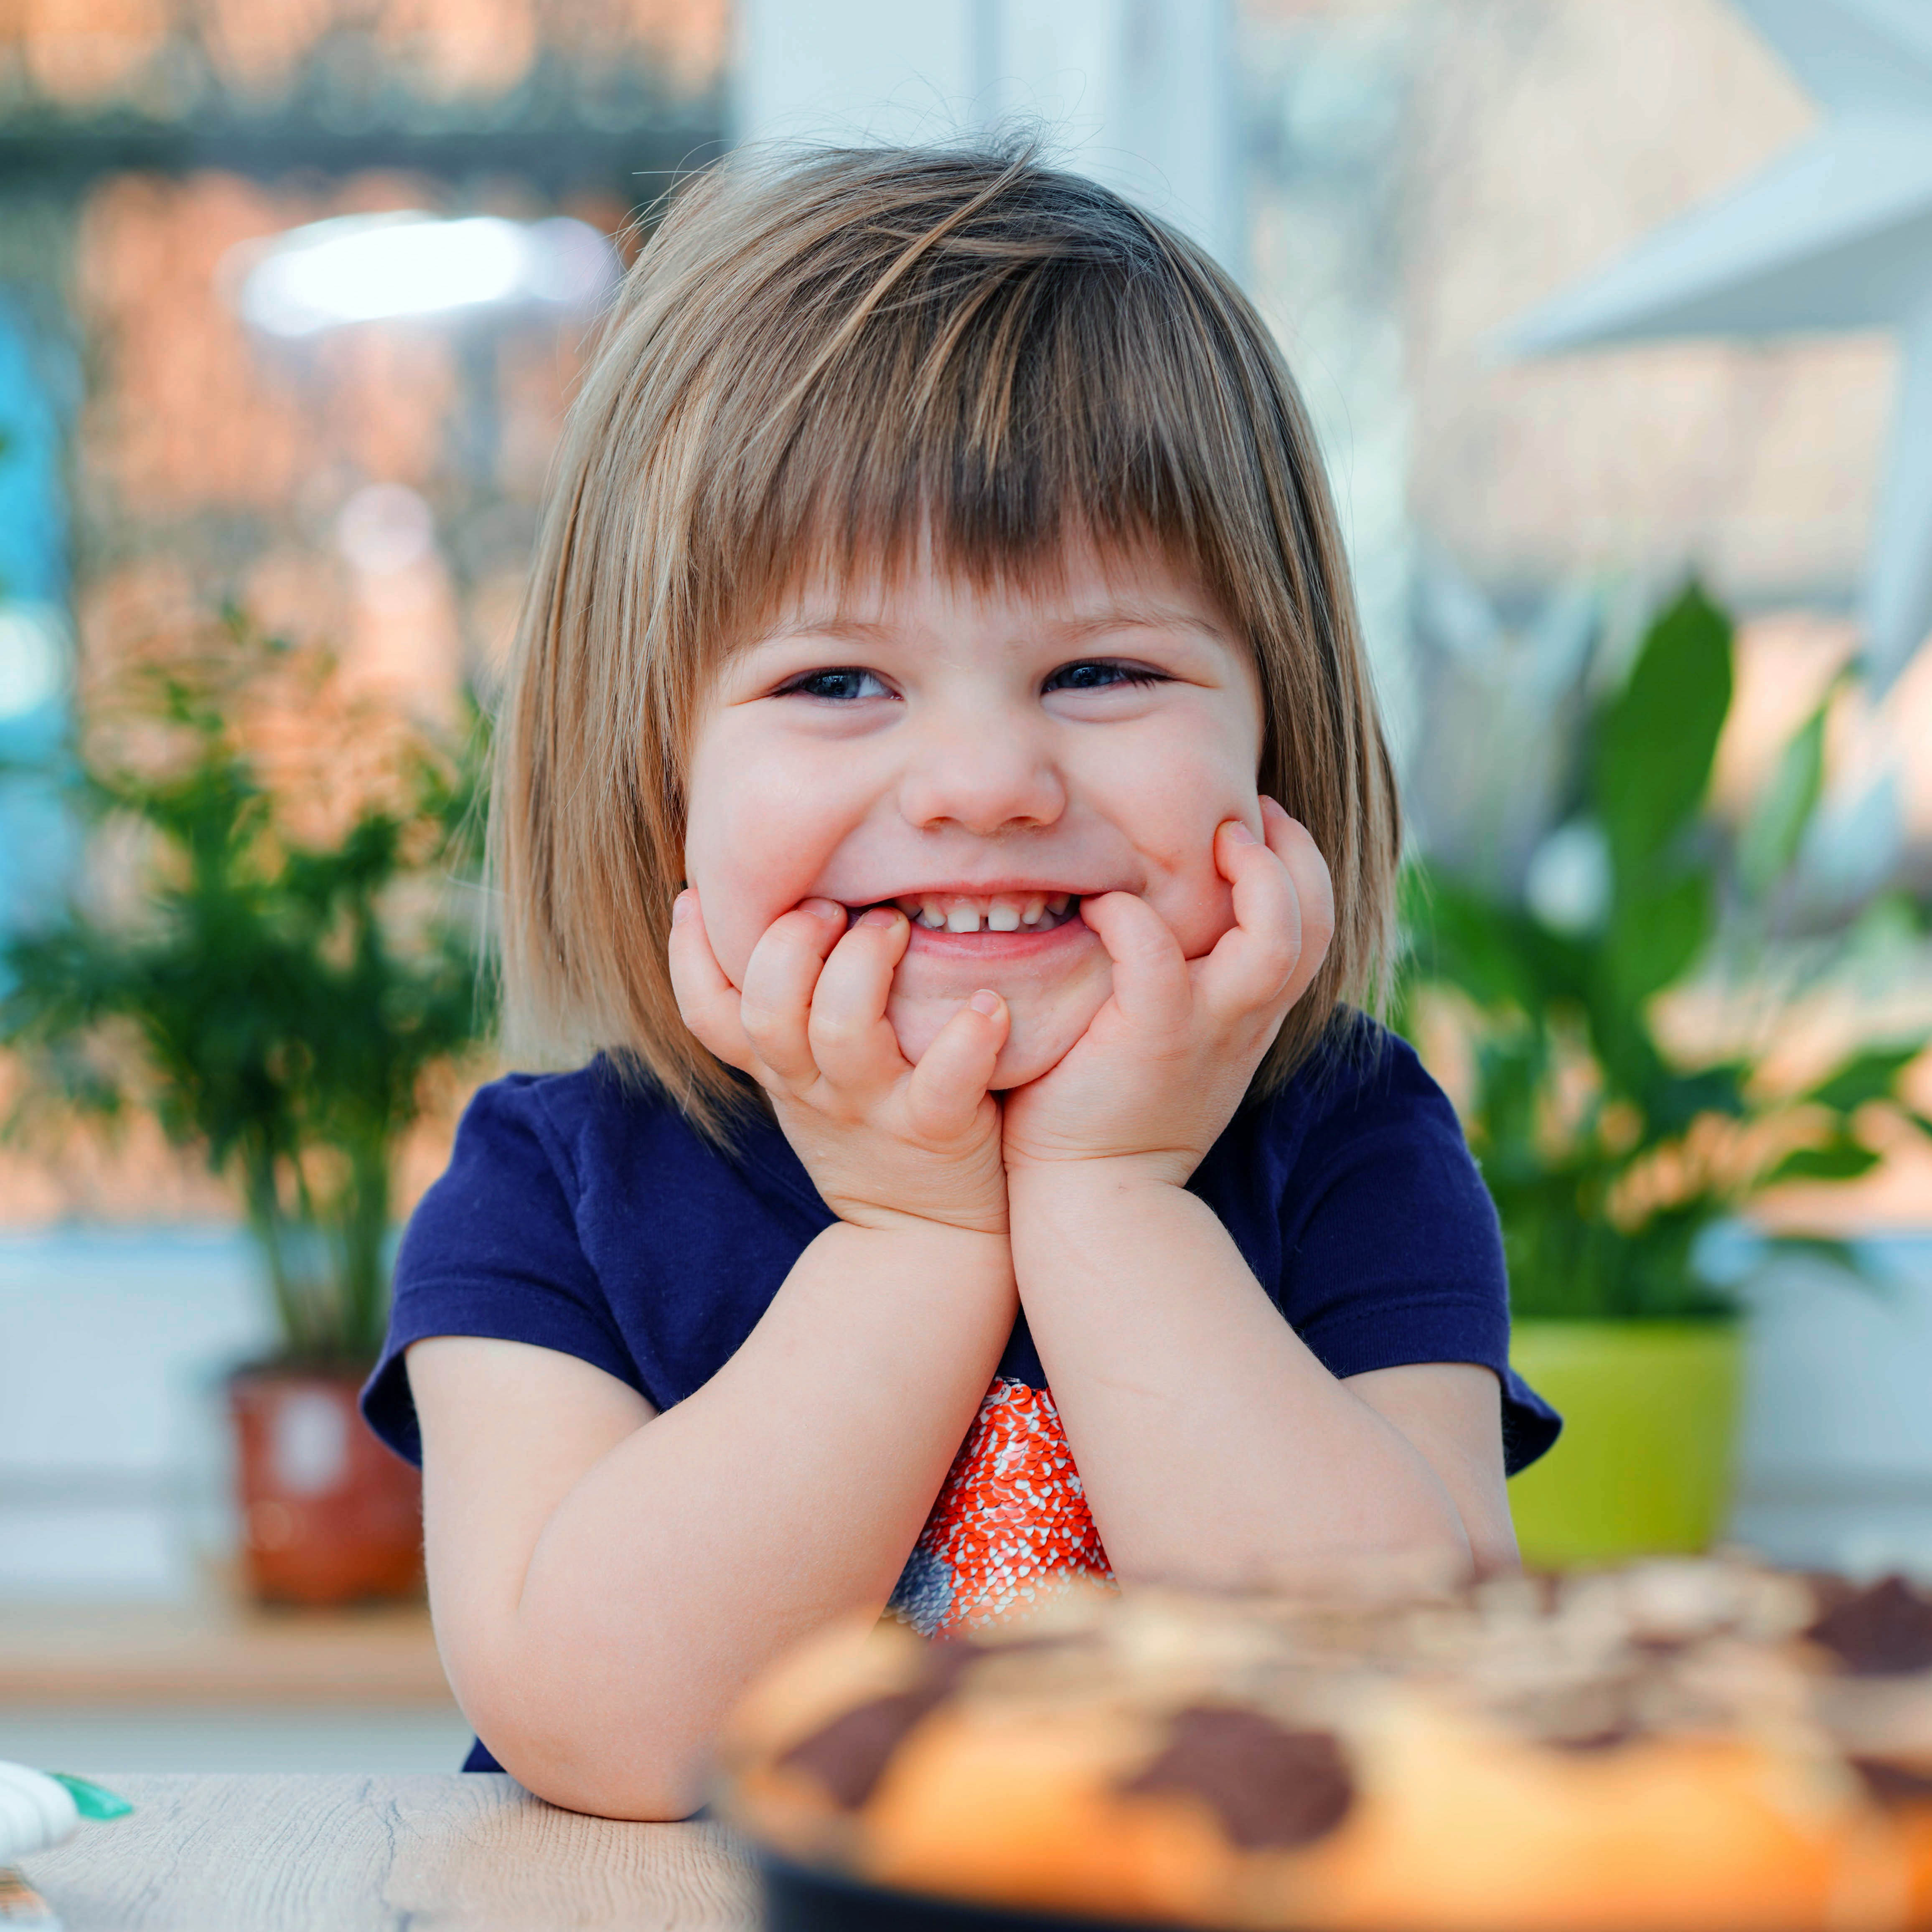
\includegraphics[width=2.1cm, height=2.1cm]{fig/ablation/1_ablation_input} & 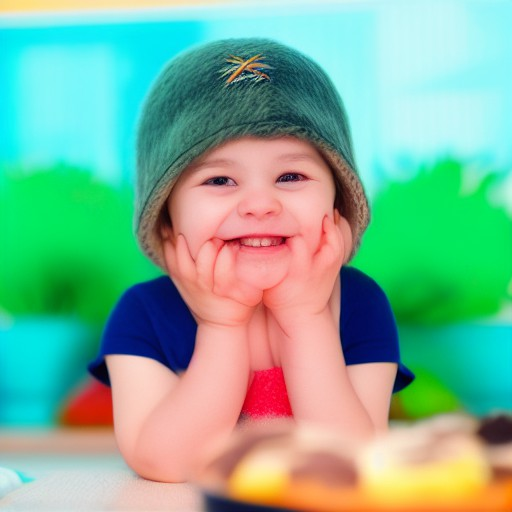
\includegraphics[width=2.1cm, height=2.1cm]{fig/ablation/1_ablation_2} &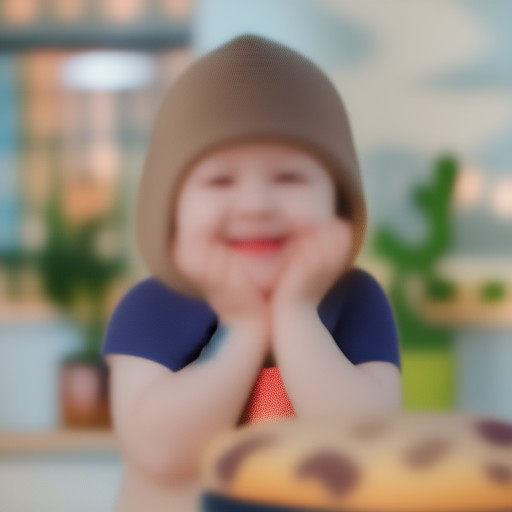
\includegraphics[width=2.1cm, height=2.1cm]{fig/ablation/1_ablation_3} &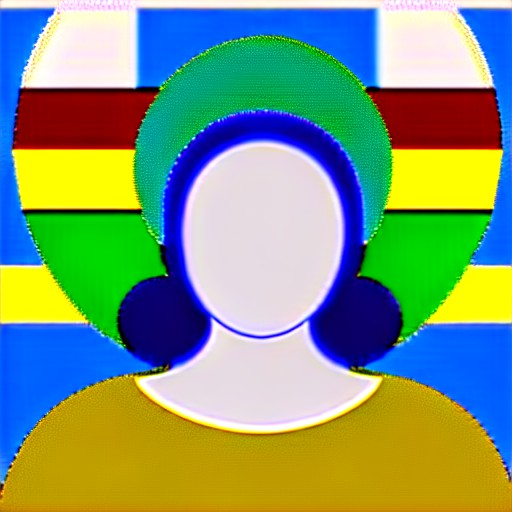
\includegraphics[width=2.1cm, height=2.1cm]{fig/ablation/1_ablation_4_cfg75} &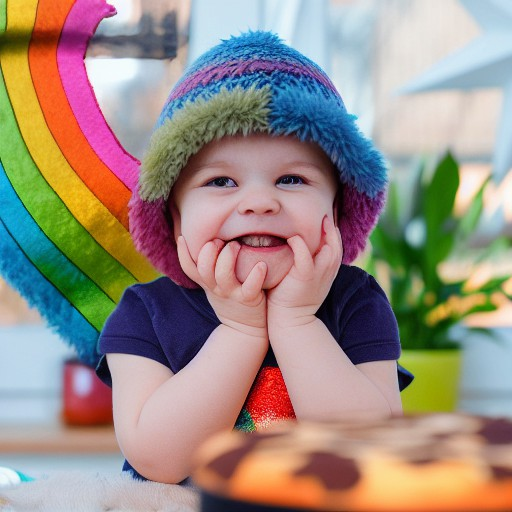
\includegraphics[width=2.1cm, height=2.1cm]{fig/ablation/1_ablation_1} &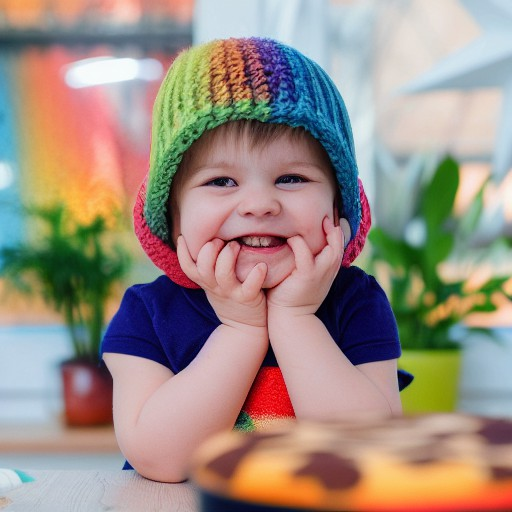
\includegraphics[width=2.1cm, height=2.1cm]{fig/ablation/1_ablation_5} &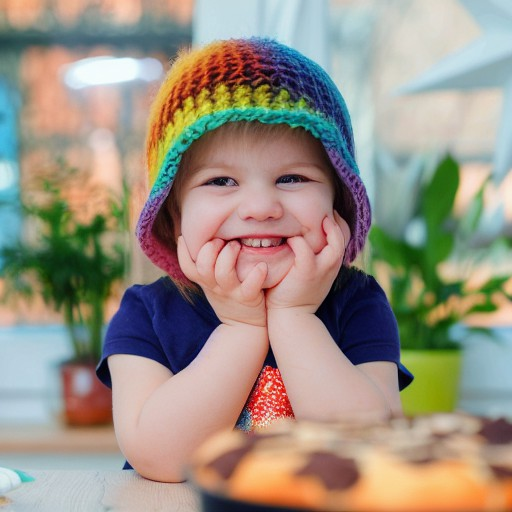
\includegraphics[width=2.1cm, height=2.1cm]{fig/ablation/1_ablation_6} \\
      \multicolumn{7}{c}{``\textit{a baby with a stuffed \textcolor{BrickRed}{\st{monkey}} \textcolor{RoyalBlue}{\textbf{zebra}} in a car}"} \\
      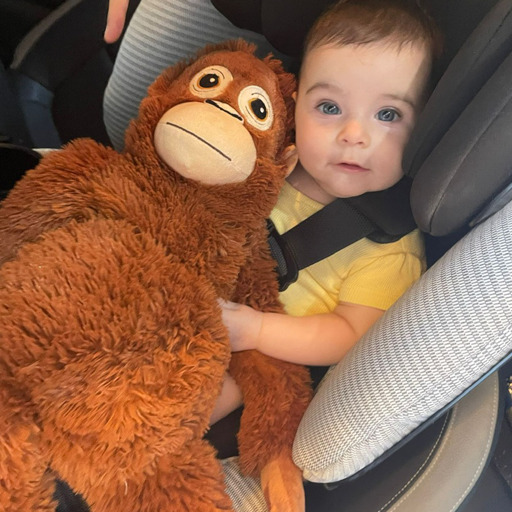
\includegraphics[width=2.1cm, height=2.1cm]{fig/ablation/0_ablation_input} & 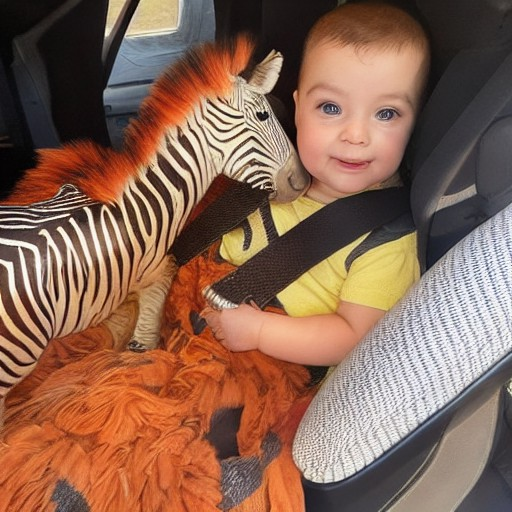
\includegraphics[width=2.1cm, height=2.1cm]{fig/ablation/0_ablation_2} &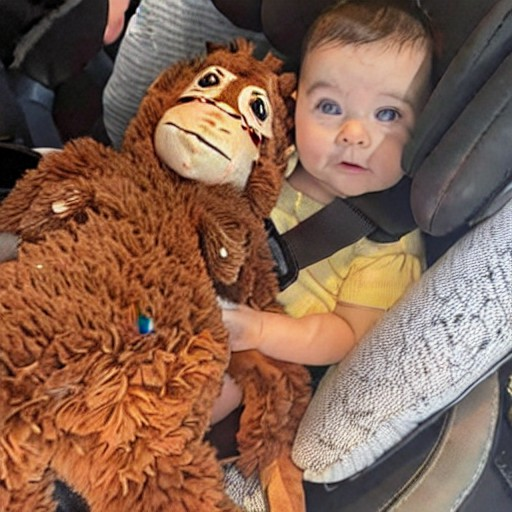
\includegraphics[width=2.1cm, height=2.1cm]{fig/ablation/0_ablation_3} &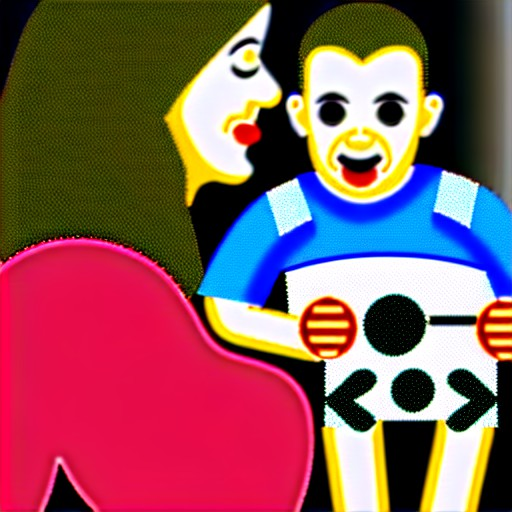
\includegraphics[width=2.1cm, height=2.1cm]{fig/ablation/0_ablation_4}
      &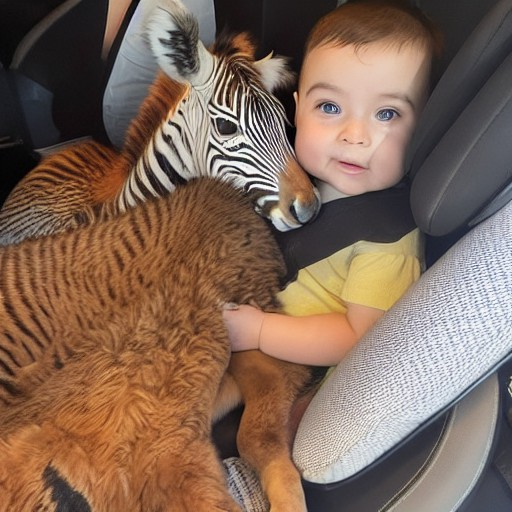
\includegraphics[width=2.1cm, height=2.1cm]{fig/ablation/0_ablation_1} &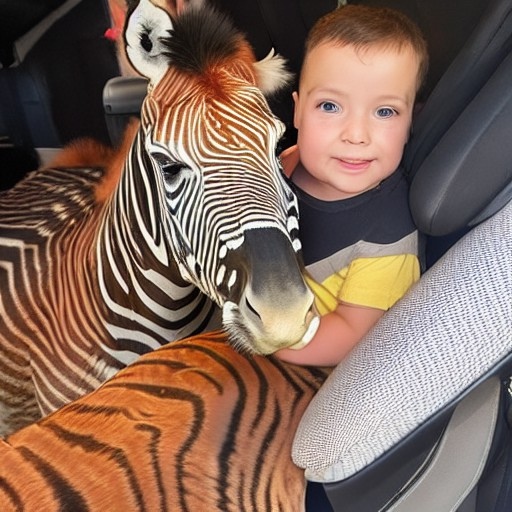
\includegraphics[width=2.1cm, height=2.1cm]{fig/ablation/0_ablation_5} &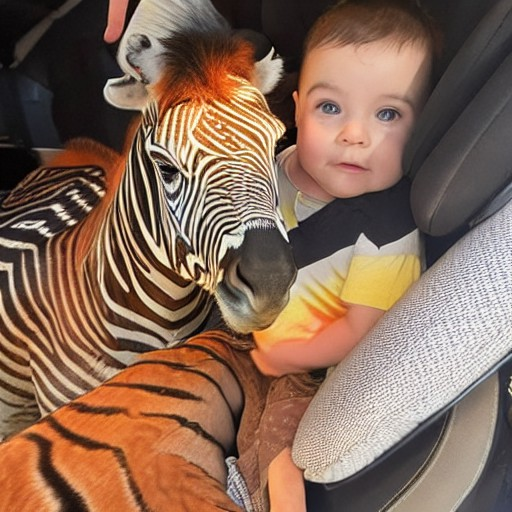
\includegraphics[width=2.1cm, height=2.1cm]{fig/ablation/0_ablation_6} \\
      \hline
      % ... Add more rows as needed
    \end{tabular}
    \caption{{\modified{}Qualitative results of the} ablation study. Each column corresponds to a configuration described in Table \ref{tab:ablation_piebench}.}
    \label{fig:ablationquali}
  \end{figure*}

\subsection{Evaluation}

\paragraph{Data} {\modified{}The analysis is conducted} on PieBench \cite{ju2023direct} and MagicBrush \cite{Zhang2023MagicBrush}. PieBench contains 700 images evenly distributed across natural and artificial scenes in four categories (animal, human, indoor, and outdoor) and 10 editing tasks, including object modification, content changes, and style adjustments. Each image includes source and target prompts, edit subjects, and manually annotated masks for background-preservation evaluation (for applicable tasks).  

MagicBrush, designed for instruction-based image editing, consists of 1053 test images with editing instructions; it also supports prompt-to-prompt editing \cite{hertz2023prompt}. Unlike PieBench, it focuses on small-scale edits in photorealistic images.  

Additionally, {\modified{}high-resolution images from Pexels}\footnote{Images in \url{https://www.pexels.com/} are free for commercial use.} {\modified{}are used} for qualitative evaluation.


\paragraph{Metrics} Following {\modified{}the} PieBench evaluation protocol \cite{ju2023direct}, {\modified{}\method{} is evaluated} using three benchmark categories: \textit{1)} structure distance \cite{tumanyan2022splicing}, \textit{2)} background preservation, and \textit{3)} target-prompt fidelity. Background preservation is measured using LPIPS \cite{zhang2018perceptual} and SSIM \cite{wang2004ssim} on the masked area, while prompt fidelity is assessed via CLIP-T Similarity \cite{we2021clipsim} on the entire image and the edited region.  

Similarly, MagicBrush evaluates methods using five metrics: four for input preservation (L1 and L2 distance, CLIP-I similarity \cite{Zhang2023MagicBrush}, and Dino similarity \cite{caron2021emerging}) and one for prompt fidelity (CLIP-T similarity).

\setlength{\tabcolsep}{1pt}
\begin{figure*}[h]
  \centering
    \footnotesize
    \small
    \resizebox{0.85\textwidth}{!}{
    \begin{tabular}{ccccccccc}
      \hline
      Input & \nulltext & NPI & \negprox & PnP & \directinversion & \ptopzero & \method \\
      \hline
      \multicolumn{8}{c}{``\textit{A \textcolor{RoyalBlue}{\textbf{lego}} cat \textcolor{RoyalBlue}{\textbf{toy}} sitting next to a mirror}"} \\
      % \insertimage{cat}{input} & \insertimage{cat}{null} &\insertimage{cat}{neg} &\insertimage{cat}{prox} &  \insertimage{cat}{pnp} & \insertimage{cat}{direct}& \insertimage{cat}{zero} & \fcolorbox{teal}{teal}{\insertimage{cat}{ours_1}}  \\
      \insertimage{cat}{input} & \insertimage{cat}{null} &\insertimage{cat}{neg} &\insertimage{cat}{prox} &  \insertimage{cat}{pnp} & \insertimage{cat}{direct}& \insertimage{cat}{zero} & \insertimage{cat}{ours_1}  \\
      \multicolumn{8}{c}{``\textit{Orange van with \textcolor{BrickRed}{\st{surfboards}} \textcolor{RoyalBlue}{\textbf{flowers}} on top}"} \\
      \insertimage{van}{input} & \insertimage{van}{null} &\insertimage{van}{neg} &\insertimage{van}{prox} & \insertimage{van}{pnp} & \insertimage{van}{direct}& \insertimage{van}{zero}& \insertimage{van}{ours}  \\
      \multicolumn{8}{c}{``\textit{Meat \textcolor{BrickRed}{\st{balls}} \textcolor{RoyalBlue}{\textbf{shushi}} on white plate}"} \\
      \insertimage{meat}{input} & \insertimage{meat}{null} &\insertimage{meat}{neg} &\insertimage{meat}{prox} & \insertimage{meat}{pnp} & \insertimage{meat}{direct}& \insertimage{meat}{zero}& \insertimage{meat}{ours}  \\
      \multicolumn{8}{c}{``\textit{A \textcolor{BrickRed}{\st{woman}} \textcolor{RoyalBlue}{\textbf{storm-trooper}} with blue hair}"} \\
      \insertimage{girl}{input} & \insertimage{girl}{null} &\insertimage{girl}{neg} &\insertimage{girl}{prox} & \insertimage{girl}{pnp} & \insertimage{girl}{direct}& \insertimage{girl}{zero3}& \insertimage{girl}{ours}  \\
      \multicolumn{8}{c}{``\textit{A \textcolor{BrickRed}{\st{cat}} \textcolor{RoyalBlue}{\textbf{dog}} sitting on a wooden chair}"} \\
      \insertimage{cat2}{input} & \insertimage{cat2}{null} &\insertimage{cat2}{neg} &\insertimage{cat2}{prox} & \insertimage{cat2}{pnp} & \insertimage{cat2}{direct}& \insertimage{cat2}{zero}& \insertimage{cat2}{ours}  \\
      \hline
      % ... Add more rows as needed
    \end{tabular}
    }
    \caption{Qualitative comparison with state-of-the-art {\modified{}methods}. {\modified{}Examples are shown for} both word insertion and word swap.}

    \label{fig:method_comparison}
  \end{figure*}
\subsection{Ablation Study}
\label{sec:expablation}




\begin{table}[htbp]
    \centering
    \small
      \renewcommand\arraystretch{0.8}
      \setlength{\tabcolsep}{0.5mm}{
    \resizebox{\linewidth}{!}{
    \begin{tabular}{llcccccc}
     \toprule
          &\multirow{2}{*}{\textbf{Reconstruction}}&\textbf{CA}&\multirow{2}{*}{\textbf{LB}}&\multirow{2}{*}{ \textbf{Struct.}$\downarrow$}      &  \multirow{2}{*}{\textbf{LPIPS} $\downarrow$}     & \multirow{2}{*}{\textbf{CLIP} $\uparrow$} \\ 
 & & \textbf{replace.}&&&&\\
    \midrule
    
    (i)&CA guidance &- & -& 15.7 & 58 & 21.9 \\
    (ii)&$\vz_t$ guidance &-& -& 40.0 & 111.3 & 21.5 \\
    (iii)&SA replace &- & -&178.4 & 376.0 & 18.8 \\
    (iv)& SA guidance& -& -&  15.7 & 42.0 & \textbf{22.0}  \\
    \midrule
    (v)& SA guidance&\checkmark&- & 14.7 & 49.5 & 21.9 \\
    (vi)& SA guidance&\checkmark&\checkmark & \textbf{11.0} & \textbf{39.6} & \textbf{22.0}\\
    \bottomrule
    \end{tabular}}
  
    }
        % \vspace{-0.2cm}
        \caption{Quantitative analysis performed on PieBench \cite{ju2023direct}. {\modified{}Four strategies (i–iv) are evaluated} for guiding reconstruction, based on either guidance or replacement, applied to the cross-attention (CA) or self-attention (SA) layers. {\modified{}Additionally, (v) CA replacement and (vi) Local Blending (LB) are evaluated} in combination with the best reconstruction approach.}
            \label{tab:ablation_piebench}
        % \vspace{-0.2cm}
    \end{table}

% \begin{table}[htbp]
%     \centering
%     \small
%       \renewcommand\arraystretch{0.8}
%       \setlength{\tabcolsep}{0.3mm}{
%     \begin{threeparttable}
%     \begin{tabular}{lccc}
 
%     \toprule
%           & \textbf{Struct.} $_{^{\times 10^3}}$ $\downarrow$    &  \textbf{LPIPS}$_{^{\times 10^3}}$ $\downarrow$     & \textbf{CLIP} $\uparrow$ \\ 
%     % \textbf{Method}            & \textbf{Distance}$_{^{\times 10^3}}$ $\downarrow$ & \textbf{PSNR} $\uparrow$     & \textbf{LPIPS}$_{^{\times 10^3}}$ $\downarrow$  & \textbf{MSE}$_{^{\times 10^4}}$ $\downarrow$     & \textbf{SSIM}$_{^{\times 10^2}}$ $\uparrow$    & \textbf{Whole}  $\uparrow$          & \textbf{Edited}  $\uparrow$       \\ \midrule
%     % \textbf{Null-text} \cite{mokady2023null} & 13.44           & 27.03  & 60.67  & 35.86  & 84.11 & 24.75        & 21.86          \\
%     % \textbf{Negative prompt} \cite{miyake2023negative} &     16.17       &  26.21 &  69.01  &  39.73 & 83.40 &   24.61     &    21.87     \\
%     % \textbf{Direct inversion} \cite{ju2023direct} & 11.65           & 27.22  & 54.55  & 32.86  & 84.76 & 25.02         & 22.10          \\
%     % \textbf{P2P-Zero} \cite{parmar2023zero} & 61.68 & 20.44  & 172.22 & 144.12 & 74.67 & 22.80 & 20.54 \\
%     % \textbf{Plug-n-Play} \cite{tumanyan2023plug} \tnote{a} & 28.22 & 22.28  & 113.46 & 83.64 & 79.05 & 25.41 & 22.55 \\
%     % \textbf{NegProx} \cite{miyake2023negative} \tnote{b} & 7.44 & 28.67 &	41.98 &	24.25 &	85.98 &	24.28 &	21.36 \\
%     % \textbf{Ours} (temporal) & 24.21 &	25.53 &	62.64 &	55.27 &	83.97 &	\textbf{26.18} &	\textbf{22.86} \\
%     % \textbf{Ours} (by task) & 12.70 &	27.67 &	42.30 &	32.09 &	85.71 &	25.75 &	22.37 \\
%     \midrule
%     Self-attn guidance\tnote{a} & 15.7 & 42.0 & \textbf{22.0}  \\
%     Cross-attn guidance\tnote{a} & 15.7 & 58 & 21.9 \\
%     Latent guidance\tnote{a} & 40.0 & 111.3 & 21.5 \\
%     \midrule
%     Self-attn replacement\tnote{a} & 178.4 & 376.0 & 18.8 \\
%     \midrule
%     Cross-attn replacement & 14.7 & 49.5 & 21.9 \\
%     Local blending\tnote{b} & \textbf{11.0} & \textbf{39.6} & \textbf{22.0}\\
%     \bottomrule

%     \end{tabular}
%     \begin{tablenotes}
%        \footnotesize
%        \item[a] Without cross-attention manipulation described in \ref{sec:cross_attention_manipulation}
%        \item[b] Including cross-attention replacement
%         \end{tablenotes}
%     \end{threeparttable}
%     }
%         \vspace{-0.2cm}
%     \caption{Quantitative analysis performed on PieBench \cite{ju2023direct}.}
%             \label{tab:ablation_piebench}
%         \vspace{-0.2cm}
%     \end{table}
    

In this ablation study, {\modified{}the evaluation begins} with the mechanism used for achieving reconstruction in the regions that should be preserved through editing. {\modified{}Four baselines are included}, employing either guidance or replacement applied to the cross-attention (CA) or self-attention (SA) layers. The baselines are as follows: (i) guidance based on CA map reconstruction, similar to \cite{parmar2023zero}, and (ii) computing the guidance term in the latent space of the diffusion model, referred to as $\vz_t$ guidance. For SA, {\modified{}two approaches are explored}: (iii) replacement as in \cite{hertz2023prompt,mokady2023null}, and (iv) guidance methods. The proposed method is an enhanced version of (iv), which {\modified{}is further refined} by sequentially integrating: (v) CA replacement, and (vi) Local blending, as detailed in Sec~\ref{sec:cross_attention_manipulation}.


The quantitative results are reported in Table \ref{tab:ablation_piebench}. Due to space constraints and the high correlation among background preservation metrics, {\modified{}the evaluation focuses} on reporting structure distance, LPIPS, and CLIP similarity, specifically in the edited areas. Complementing this quantitative evaluation, {\modified{}the qualitative examples} in Fig.~\ref{fig:ablationquali} {\modified{}showcase} results obtained using the exact same baselines.



Among the various reconstruction mechanisms evaluated, guidance-based approaches (i, ii, and iv) consistently outperform the replacement strategy (iii) across all metrics. This superiority is also reflected qualitatively in Fig.~\ref{fig:ablationquali}, where images resulting from SA replacement are notably unrealistic and diverge from the original. While CA guidance (i) yields satisfactory results, it falls behind {\modified{}the proposed SA guidance} approach by 16 points in the LPIPS metric. Qualitatively, this drop in reconstruction is clearly noticeable in the first row of Fig.~\ref{fig:ablationquali}. Finally, $\vz_t$ guidance (ii) lags behind both in quantitative and qualitative terms compared to the other guidance methods.



{\modified{}Regarding CA replacement (v), observations reveal} that although there is a slight increase in LPIPS, it is compensated by improved structure preservation metrics. This qualitative enhancement is particularly evident in the first row of Fig.~\ref{fig:ablationquali}, where the background preservation is notably better. In (vi), Local Blending (LB) improves both the structure metric and LPIPS, without compromising the CLIP metric. This effectively demonstrates the capability of {\modified{}the LB mechanism} to maintain editability while preserving structural integrity, as it only affects areas unrelated to the editing.


\subsection{Comparison with the State-of-the-Art}

% \begin{table*}[htbp]
%     \centering
%       \renewcommand\arraystretch{0.9}
%       \setlength{\tabcolsep}{0.3mm}{
%     \begin{threeparttable}
%     \begin{tabular}{c|c|cccc|cc}
%     \toprule
%     \toprule
%           & \textbf{Structure}          & \multicolumn{4}{c|}{\textbf{Background Preservation}} & \multicolumn{2}{c}{\textbf{CLIP Similariy}} \\ \midrule
%     \textbf{Method}            & \textbf{Distance}$_{^{\times 10^3}}$ $\downarrow$ & \textbf{PSNR} $\uparrow$     & \textbf{LPIPS}$_{^{\times 10^3}}$ $\downarrow$  & \textbf{MSE}$_{^{\times 10^4}}$ $\downarrow$     & \textbf{SSIM}$_{^{\times 10^2}}$ $\uparrow$    & \textbf{Whole}  $\uparrow$          & \textbf{Edited}  $\uparrow$       \\ \midrule
%     \textbf{Null-text} \cite{mokady2023null} & 13.44           & 27.03  & 60.67  & 35.86  & 84.11 & 24.75        & 21.86          \\
%     \textbf{Negative prompt} \cite{miyake2023negative} &     16.17       &  26.21 &  69.01  &  39.73 & 83.40 &   24.61     &    21.87     \\
%     \textbf{Direct inversion} \cite{ju2023direct} & 11.65           & 27.22  & 54.55  & 32.86  & 84.76 & 25.02         & \textbf{22.10}          \\
%     \textbf{P2P-Zero} \cite{parmar2023zero} & 61.68 & 20.44  & 172.22 & 144.12 & 74.67 & 22.80 & 20.54 \\
%     \textbf{Plug-n-Play} \cite{tumanyan2023plug} \tnote{a} & 28.22 & 22.28  & 113.46 & 83.64 & 79.05 & 25.41 & 22.55 \\
%     \textbf{NegProx} \cite{miyake2023negative} \tnote{b} & \textbf{7.44} & \textbf{28.67} &	41.98 &	\textbf{24.25} &	\textbf{85.98} &	24.28 &	21.36 \\
%     % \textbf{Ours} (temporal) & 24.21 &	25.53 &	62.64 &	55.27 &	83.97 &	\textbf{26.18} &	\textbf{22.86} \\
%     \textbf{Ours} & 10.96 &	27.91 &	\textbf{39.56} &	29.80 &	85.97 &	\textbf{25.47} &	21.96 \\
%     \textbf{Ours} (by task) & 12.70 &	27.67 &	42.30 &	32.09 &	85.71 &	25.75 &	22.37 \\
    
%     \bottomrule
%     \bottomrule
%     \end{tabular}
%     \begin{tablenotes}
%        \footnotesize
%        \item[a] use Stable Diffusion v1.5 as base model (others all use Stable Diffusion v1.4) %revise the source code's 1000 steps to 50 steps
%        \item[b] Proximal guidance with negative prompt as introduced in \cite{han2023proximal}
%         \end{tablenotes}
%     \end{threeparttable}
%     }
%         \vspace{-0.2cm}
%     \caption{Quantitutive analysis performed on PieBench \cite{ju2023direct}. All rows but ours are taken from \cite{ju2023direct}.}
%             \label{tab:comparison_piebench}
%         \vspace{-0.2cm}
%     \end{table*}
    

% \begin{table*}[htbp]
%     \centering
%     \small
%       \renewcommand\arraystretch{0.9}
%       \setlength{\tabcolsep}{0.3mm}{
%     \begin{threeparttable}
%     \begin{tabular}{cccccc}
%    % \toprule
%     \toprule
%           & \textbf{Struct.}          & \multicolumn{2}{c|}{\textbf{Background Preservation}} & \multicolumn{2}{c}{\textbf{CLIP Similariy}} \\ \midrule
%     \textbf{Method}            & \textbf{Distance}$_{^{\times 10^3}}$ $\downarrow$ &   \textbf{LPIPS}$_{^{\times 10^3}}$ $\downarrow$  & \textbf{SSIM}$_{^{\times 10^2}}$ $\uparrow$    & \textbf{Whole}  $\uparrow$          & \textbf{Edited}  $\uparrow$       \\ \midrule
%     \textbf{\nulltextlong} \cite{mokady2023null} & 13.4             & 60.7    & 84.1 & 24.8        & 21.9          \\
%     \textbf{Negative prompt} \cite{miyake2023negative} &     16.2        &  69.0   & 83.4 &   24.6     &    21.9     \\
%     \textbf{\directinversionlong} \cite{ju2023direct} & 11.7             & 54.6    & 84.8 & 25.0         & 22.1          \\
%     \textbf{\ptopzerolong} \cite{parmar2023zero} & 61.7   & 172.2 & 74.7 & 22.8 & 20.5 \\
%     \textbf{\pnplong} \cite{tumanyan2023plug} \tnote{a} & 28.2   & 113.5 & 79.0 & 25.4 & \textbf{22.6} \\
%     \textbf{\negproxlong} \cite{miyake2023negative} \tnote{b} & \textbf{7.4}  &	42.0  &	\textbf{86.0} &	24.3 &	21.4 \\
%     % \textbf{Ours} (temporal) & 24.21 &	25.53 &	62.64 &	55.27 &	83.97 &	\textbf{26.18} &	\textbf{22.86} \\
%     \textbf{\method} (ours) & 11.0 &	\textbf{39.6} &	\textbf{86.0} &	\textbf{25.5} &	22.0 \\
%     % \textbf{Ours} (by task) & 12.70 &	42.30  &	85.71 &	25.75 &	22.37 \\
    
%     \bottomrule
%     %\bottomrule
%     \end{tabular}
%     \begin{tablenotes}
%        \footnotesize
%        \item[a] use Stable Diffusion v1.5 as base model (others all use Stable Diffusion v1.4) %revise the source code's 1000 steps to 50 steps
%        \item[b] Proximal guidance with negative prompt as introduced in \cite{han2023proximal}
%         \end{tablenotes}
%     \end{threeparttable}
%     }
%         \vspace{-0.2cm}
%     \caption{Quantitative analysis performed on PieBench \cite{ju2023direct}. All rows but ours are taken from \cite{ju2023direct}.}
%             \label{tab:comparison_piebench}
%         \vspace{-0.2cm}
%     \end{table*}




    \begin{table}[htbp]
    \centering
    \small
      \renewcommand\arraystretch{0.9}
      \setlength{\tabcolsep}{0.5mm}{
  \resizebox{\linewidth}{!}{  \begin{tabular}{cccccc}
   % \toprule
    \toprule
          & \textbf{Struct.}          & \multicolumn{2}{c}{\textbf{BG}} & \multicolumn{2}{c}{\textbf{CLIP-T Similariy}} \\ \midrule
    \textbf{Method}            & \textbf{Dist.} $\downarrow$ &   \textbf{LPIPS} $\downarrow$  & \textbf{SSIM} $\uparrow$    & \textbf{Whole}  $\uparrow$          & \textbf{Edited}  $\uparrow$       \\ \midrule
    \textbf{\nulltextlong} \cite{mokady2023null} & 13.4             & 60.7    & 84.1 & 24.8        & 21.9          \\
    \textbf{Negative prompt} \cite{miyake2023negative} &     16.2        &  69.0   & 83.4 &   24.6     &    21.9     \\
    \textbf{\negproxlong} \cite{miyake2023negative}  & \textbf{7.4}  &	42.0  &	\textbf{86.0} &	24.3 &	21.4 \\
    \textbf{\pnplong} \cite{tumanyan2023plug}  & 28.2   & 113.5 & 79.0 & 25.4 & \textbf{22.6} \\
    \textbf{\directinversionlong} \cite{ju2023direct} & 11.7             & 54.6    & 84.8 & 25.0         & 22.1          \\
    \textbf{\ptopzerolong} \cite{parmar2023zero} & 61.7   & 172.2 & 74.7 & 22.8 & 20.5 \\
    \textbf{\method} (ours) & 11.0 &	\textbf{39.6} &	\textbf{86.0} &	\textbf{25.5} &	22.0 \\
    
    \bottomrule
    %\bottomrule
    \end{tabular}}

    }
        % \vspace{-0.2cm}
        \caption{Quantitative analysis performed on PieBench. All rows but ours are taken directly from the \directinversion{} work \cite{ju2023direct}. BG stands for Background.}
            \label{tab:comparison_piebench}
        % \vspace{-0.2cm}
    \end{table}


  

% \begin{table*}[htbp]
%     \centering
%       \renewcommand\arraystretch{0.9}
%       \setlength{\tabcolsep}{0.3mm}{
%     \begin{threeparttable}
%     \begin{tabular}{c|c|cccc|cc}
%     \toprule
%     \toprule
%           & \textbf{Structure}          & \multicolumn{4}{c|}{\textbf{Background Preservation}} & \multicolumn{2}{c}{\textbf{CLIP Similariy}} \\ \midrule
%     \textbf{Method}            & \textbf{Distance}$_{^{\times 10^3}}$ $\downarrow$ & \textbf{PSNR} $\uparrow$     & \textbf{LPIPS}$_{^{\times 10^3}}$ $\downarrow$  & \textbf{MSE}$_{^{\times 10^4}}$ $\downarrow$     & \textbf{SSIM}$_{^{\times 10^2}}$ $\uparrow$    & \textbf{Whole}  $\uparrow$          & \textbf{Edited}  $\uparrow$       \\ \midrule
%     \textbf{Null-text} \cite{mokady2023null} & 13.44           & 27.03  & 60.67  & 35.86  & 84.11 & 24.75        & 21.86          \\
%     \textbf{Negative prompt} \cite{miyake2023negative} &     16.17       &  26.21 &  69.01  &  39.73 & 83.40 &   24.61     &    21.87     \\
%     \textbf{Direct inversion} \cite{ju2023direct} & 11.65           & 27.22  & 54.55  & 32.86  & 84.76 & 25.02         & \textbf{22.10}          \\
%     \textbf{P2P-Zero} \cite{parmar2023zero} & 61.68 & 20.44  & 172.22 & 144.12 & 74.67 & 22.80 & 20.54 \\
%     \textbf{Plug-n-Play} \cite{tumanyan2023plug} \tnote{a} & 28.22 & 22.28  & 113.46 & 83.64 & 79.05 & 25.41 & 22.55 \\
%     \textbf{NegProx} \cite{miyake2023negative} \tnote{b} & \textbf{7.44} & \textbf{28.67} &	41.98 &	\textbf{24.25} &	\textbf{85.98} &	24.28 &	21.36 \\
%     % \textbf{Ours} (temporal) & 24.21 &	25.53 &	62.64 &	55.27 &	83.97 &	\textbf{26.18} &	\textbf{22.86} \\
%     \textbf{Ours} & 10.96 &	27.91 &	\textbf{39.56} &	29.80 &	85.97 &	\textbf{25.47} &	21.96 \\
%     \textbf{Ours} (by task) & 12.70 &	27.67 &	42.30 &	32.09 &	85.71 &	25.75 &	22.37 \\
    
%     \bottomrule
%     \bottomrule
%     \end{tabular}
%     \begin{tablenotes}
%        \footnotesize
%        \item[a] use Stable Diffusion v1.5 as base model (others all use Stable Diffusion v1.4) %revise the source code's 1000 steps to 50 steps
%        \item[b] Proximal guidance with negative prompt as introduced in \cite{han2023proximal}
%         \end{tablenotes}
%     \end{threeparttable}
%     }
%         \vspace{-0.2cm}
%     \caption{Quantitutive analysis performed on PieBench \cite{ju2023direct}. All rows but ours are taken from \cite{ju2023direct}.}
%             \label{tab:comparison_piebench}
%         \vspace{-0.2cm}
%     \end{table*}
    

% \begin{table*}[htbp]
%     \centering
%     \small
%       \renewcommand\arraystretch{0.9}
%       \setlength{\tabcolsep}{0.3mm}{
%     \begin{threeparttable}
%     \begin{tabular}{cccccc}
%    % \toprule
%     \toprule
%           & \textbf{Struct.}          & \multicolumn{2}{c|}{\textbf{Background Preservation}} & \multicolumn{2}{c}{\textbf{CLIP Similariy}} \\ \midrule
%     \textbf{Method}            & \textbf{Distance}$_{^{\times 10^3}}$ $\downarrow$ &   \textbf{LPIPS}$_{^{\times 10^3}}$ $\downarrow$  & \textbf{SSIM}$_{^{\times 10^2}}$ $\uparrow$    & \textbf{Whole}  $\uparrow$          & \textbf{Edited}  $\uparrow$       \\ \midrule
%     \textbf{\nulltextlong} \cite{mokady2023null} & 13.4             & 60.7    & 84.1 & 24.8        & 21.9          \\
%     \textbf{Negative prompt} \cite{miyake2023negative} &     16.2        &  69.0   & 83.4 &   24.6     &    21.9     \\
%     \textbf{\directinversionlong} \cite{ju2023direct} & 11.7             & 54.6    & 84.8 & 25.0         & 22.1          \\
%     \textbf{\ptopzerolong} \cite{parmar2023zero} & 61.7   & 172.2 & 74.7 & 22.8 & 20.5 \\
%     \textbf{\pnplong} \cite{tumanyan2023plug} \tnote{a} & 28.2   & 113.5 & 79.0 & 25.4 & \textbf{22.6} \\
%     \textbf{\negproxlong} \cite{miyake2023negative} \tnote{b} & \textbf{7.4}  &	42.0  &	\textbf{86.0} &	24.3 &	21.4 \\
%     % \textbf{Ours} (temporal) & 24.21 &	25.53 &	62.64 &	55.27 &	83.97 &	\textbf{26.18} &	\textbf{22.86} \\
%     \textbf{\method} (ours) & 11.0 &	\textbf{39.6} &	\textbf{86.0} &	\textbf{25.5} &	22.0 \\
%     % \textbf{Ours} (by task) & 12.70 &	42.30  &	85.71 &	25.75 &	22.37 \\
    
%     \bottomrule
%     %\bottomrule
%     \end{tabular}
%     \begin{tablenotes}
%        \footnotesize
%        \item[a] use Stable Diffusion v1.5 as base model (others all use Stable Diffusion v1.4) %revise the source code's 1000 steps to 50 steps
%        \item[b] Proximal guidance with negative prompt as introduced in \cite{han2023proximal}
%         \end{tablenotes}
%     \end{threeparttable}
%     }
%         \vspace{-0.2cm}
%     \caption{Quantitative analysis performed on PieBench \cite{ju2023direct}. All rows but ours are taken from \cite{ju2023direct}.}
%             \label{tab:comparison_piebench}
%         \vspace{-0.2cm}
%     \end{table*}




    \begin{table}[htbp]
        
    \centering
    \small
      \renewcommand\arraystretch{0.9}
      \setlength{\tabcolsep}{0.5mm}{
  \resizebox{\linewidth}{!}{  \begin{tabular}{cccccc}
   % \toprule
    \toprule
        %   & \multicolumn{4}{c}{\textbf{Structure}} & \textbf{CLIP Similariy} \\ \midrule
    \textbf{Method}            & \textbf{L1} $\downarrow$ &   \textbf{L2} $\downarrow$  & \textbf{CLIP-I} $\uparrow$    & \textbf{Dino}  $\uparrow$          & \textbf{CLIP-T}  $\uparrow$       \\ \midrule
    \textbf{\negproxlong} \cite{miyake2023negative}  & 7.0  &	1.85  &	88.7 &	83.0 &	26.7 \\
    \textbf{\directinversionlong} \cite{ju2023direct} & 8.1             & 2.04    & 89.8 & 84.9         & \textbf{27.9}          \\
    \textbf{\ptopzerolong} \cite{parmar2023zero} & 17.4   & 7.6 & 80.7 & 69.3 & 26.4 \\
    \textbf{\method} (ours) & \textbf{6.4} &	\textbf{1.8} &	\textbf{90.9} &	\textbf{85.9} &	27.6 \\
    
    \bottomrule
    %\bottomrule
    \end{tabular}}

    }
        % \vspace{-0.2cm}
    \caption{    
    Quantitative analysis performed on MagicBrush. 
        }
            \label{tab:comparison_magicbrush}
        % \vspace{-0.2cm}
    \end{table}


  


\label{sec:expsota}
\paragraph{Quantitative Comparison}

{\modified{}The proposed method is compared} with state-of-the-art approaches in Tables~\ref{tab:comparison_piebench} and \ref{tab:comparison_magicbrush}. On PieBench, while \ptopzerolong{} underperforms across all metrics, methods such as \pnplong{} obtain high CLIP-T similarity by sacrificing structure and background fidelity, and although \negproxlong{} achieves the best structure fidelity, it does so at the expense of lower CLIP-T similarity. In contrast, \method{} strikes an excellent balance by delivering the best background preservation, near-top (second-best) structure fidelity, the highest Whole CLIP-T, and competitive Edited CLIP-T scores. Similarly, on MagicBrush, \method{} outperforms all alternatives across nearly every metric. These results highlight that \method{} consistently delivers robust, well-rounded performance without relying on inversion of the input image.





\paragraph{Qualitative Comparison}
\label{par:qualitative}
\setlength{\tabcolsep}{1pt}
\begin{figure}[h]
    \footnotesize
    \small
    \begin{tabularx}{\columnwidth}{ YYYYYY }
        % \cline{2-7}
        %    \multicolumn{1}{c|}{} 
        %  & \multicolumn{3}{c|}{Fantastical aardvarks}  
        %  & \multicolumn{3}{c|}{Spelunking elephants}\\
        % \hline
        %  Foo bar & A & B & C & A & B & C\\
        Input & \ptopzero &  \nulltext &  \directinversion &  \negprox &  \method \\
        \multicolumn{6}{c}{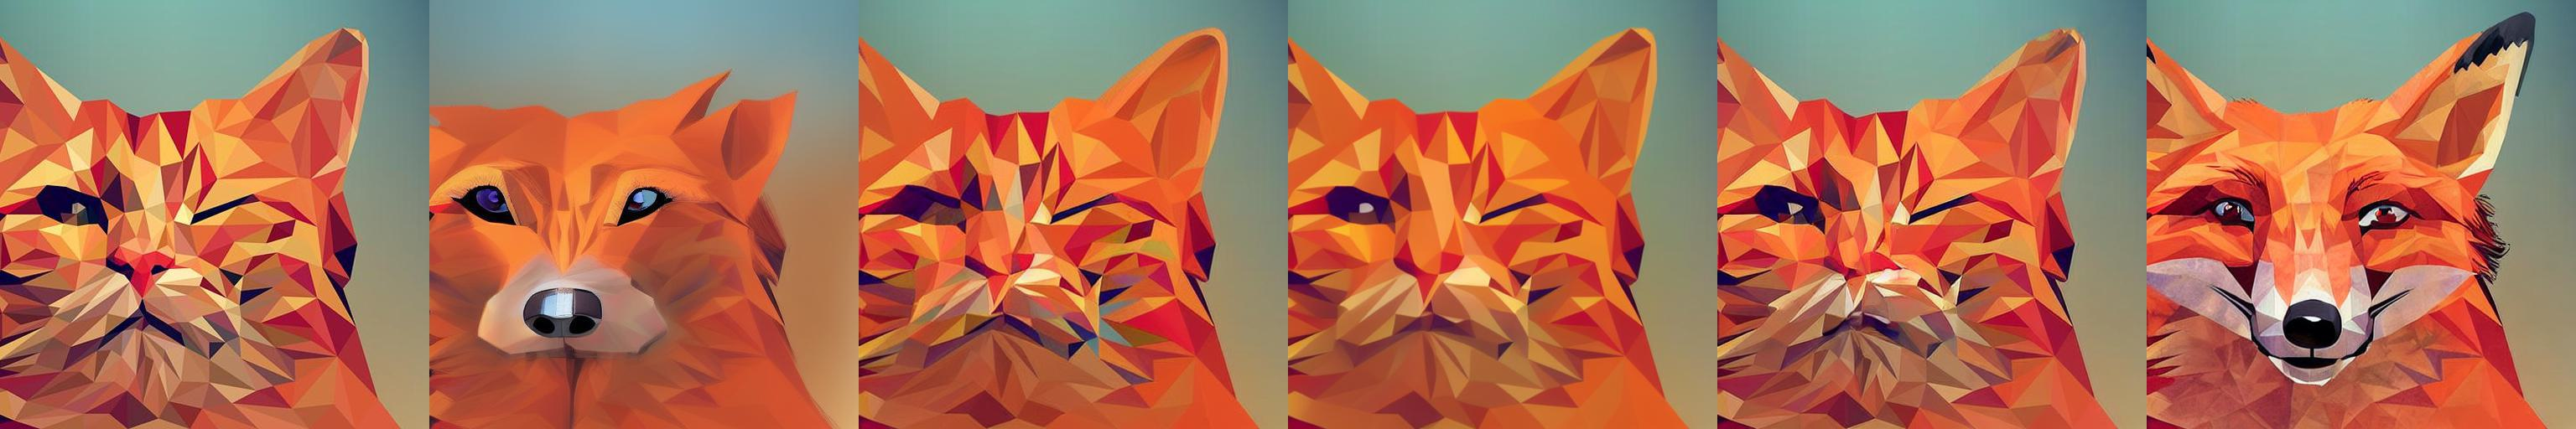
\includegraphics[width=\columnwidth]{fig/ex_all/0_random_140-000000000080}} \\
        \multicolumn{6}{c}{``\textit{a \textcolor{BrickRed}{\st{cat}} \textcolor{RoyalBlue}{\textbf{fox}} is shown in a low polygonal style}"} \\
        \multicolumn{6}{c}{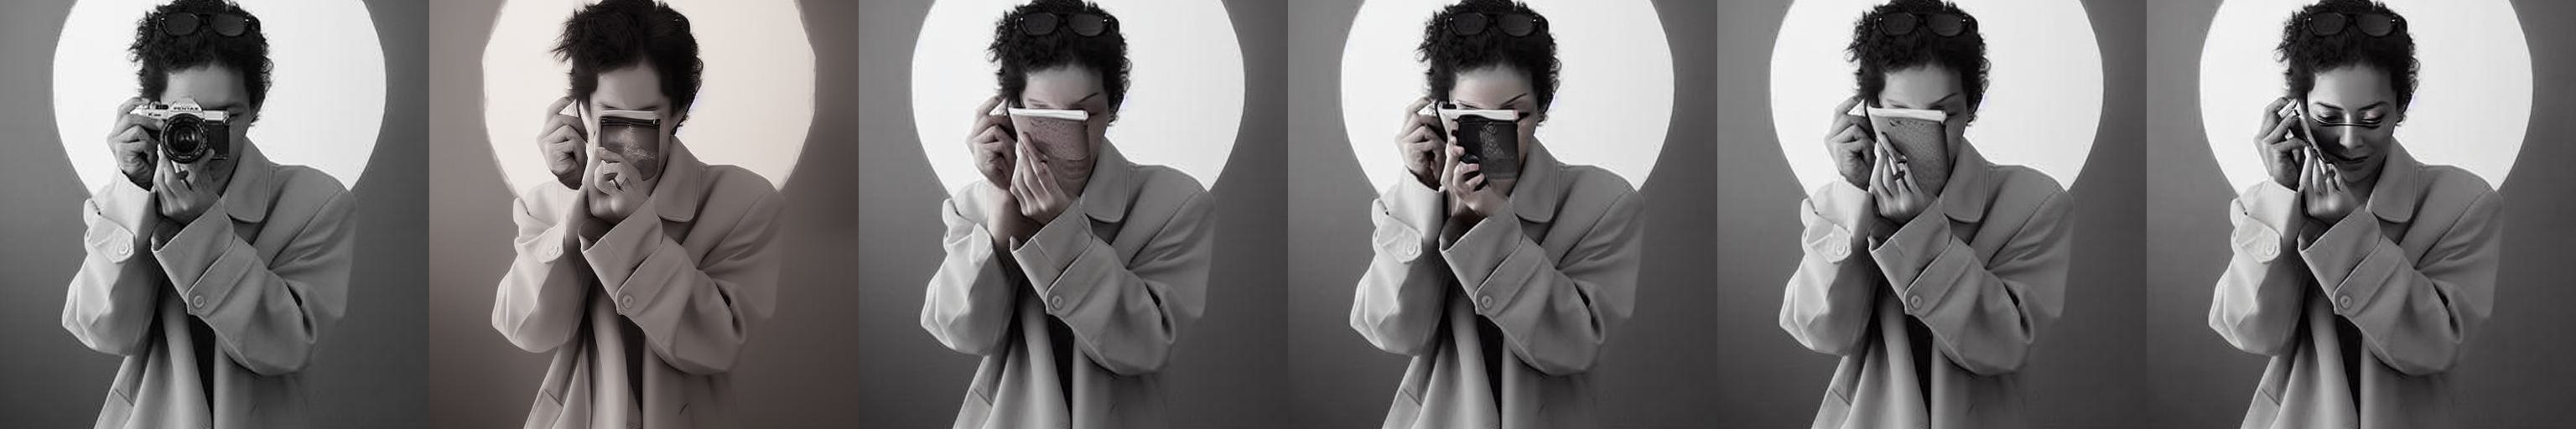
\includegraphics[width=\columnwidth]{fig/ex_all/1_change_object_80-2_natural-2_human-122000000002}} \\
        \multicolumn{6}{c}{``\textit{a woman in a coat holding a \textcolor{BrickRed}{\st{camera}} \textcolor{RoyalBlue}{\textbf{phone}} on white plate}"} \\
        \multicolumn{6}{c}{
\includegraphics[width=\columnwidth]{fig/ex_all/9_change_style_80-1_artificial-2_human-912000000001}} \\
        \multicolumn{6}{c}{``\textit{a clown \textcolor{RoyalBlue}{\textbf{in pixel art style}} with colorful hair}"} \\
        \multicolumn{6}{c}{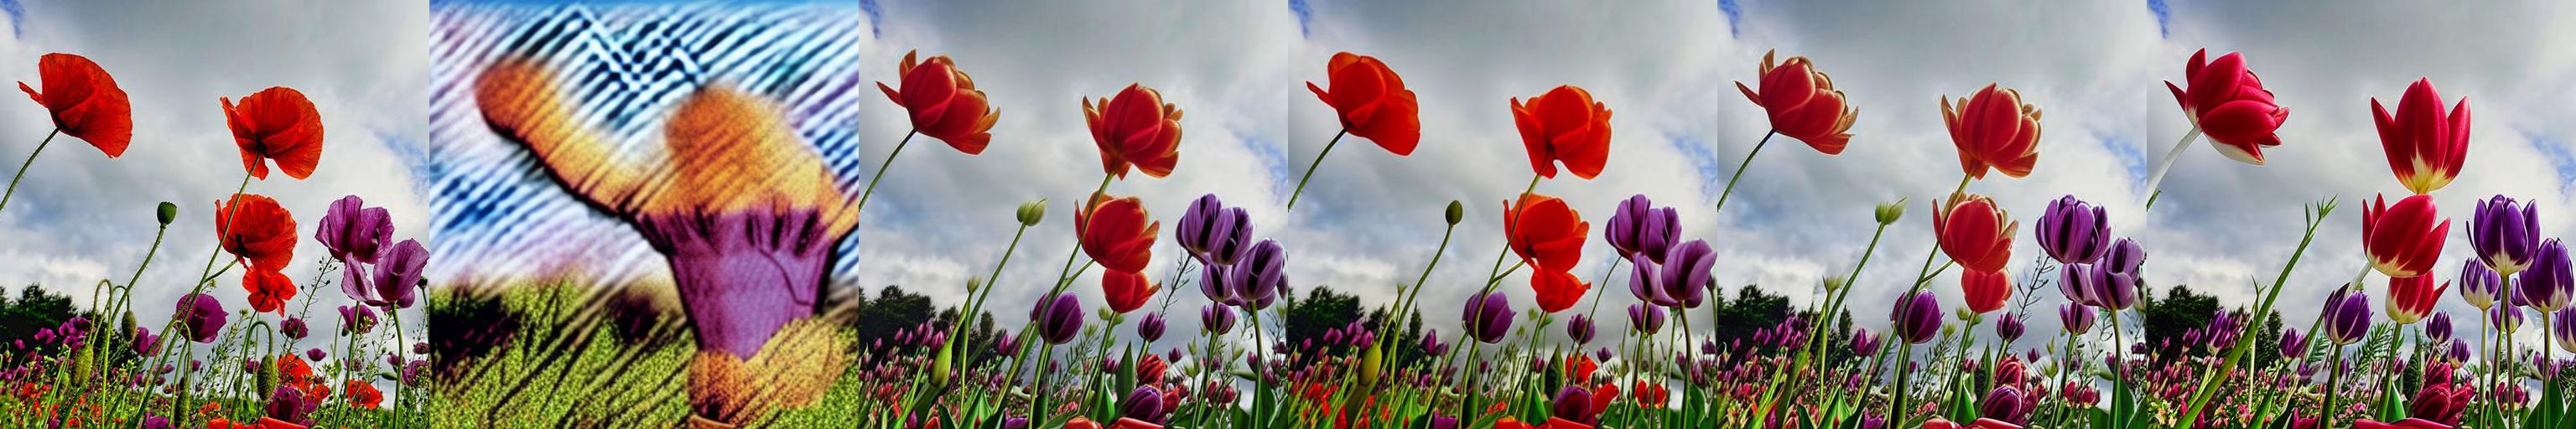
\includegraphics[width=\columnwidth]{fig/ex_all/0_random_140-000000000101}} \\
        \multicolumn{6}{c}{``\textit{\textcolor{BrickRed}{\st{poppies}} \textcolor{RoyalBlue}{\textbf{tulips}}}"} \\
        \multicolumn{6}{c}{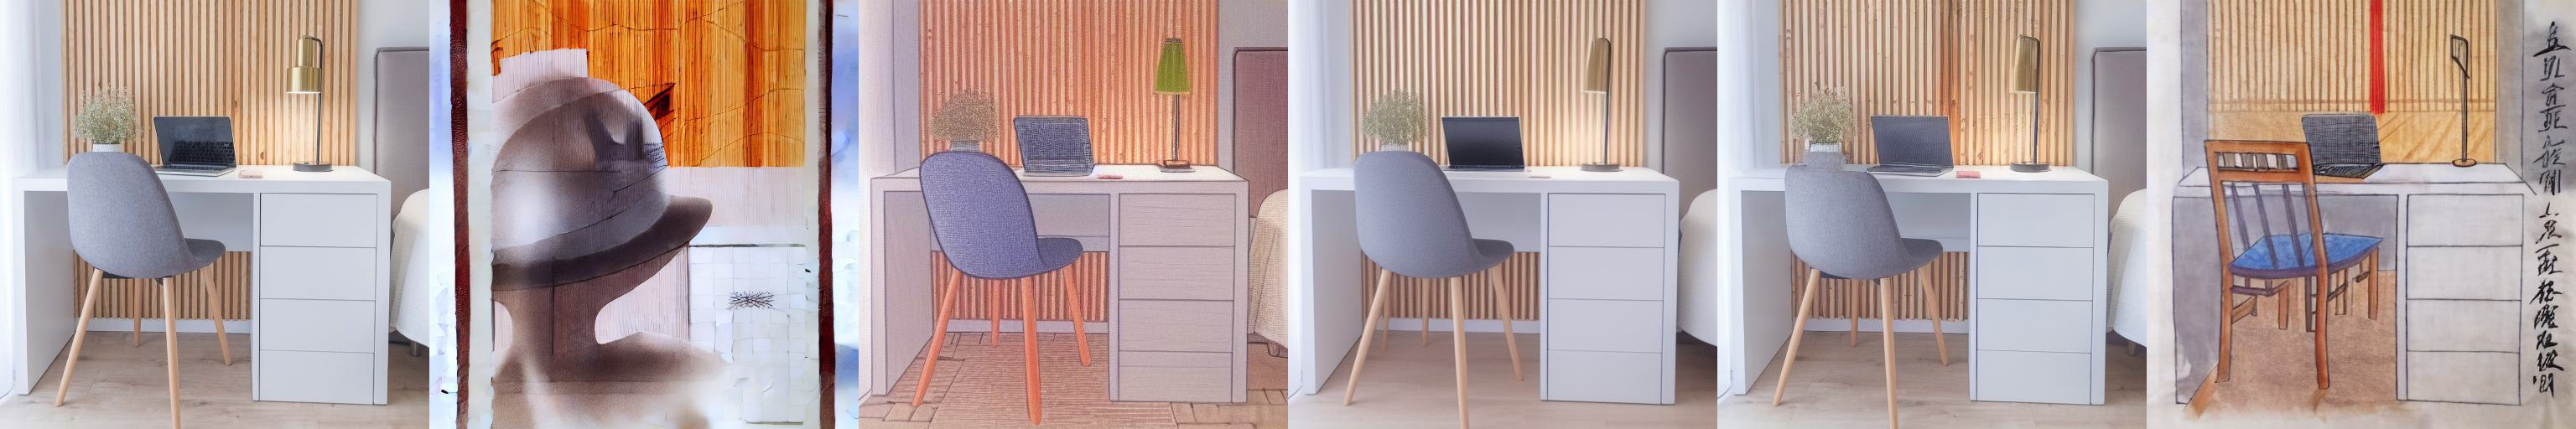
\includegraphics[width=\columnwidth]{fig/ex_all/9_change_style_80-2_natural-3_indoor-923000000007}} \\
        \multicolumn{6}{c}{``\textit{\textcolor{RoyalBlue}{\textbf{chinese painting of}} a white desk with a laptop and chair}"} \\
        \end{tabularx}
        \caption{Examples from the PieBench dataset illustrating the strengths of \method{}, including superior style transfer, content modification, and object removal.        }
    \label{fig:qual_adv}
  \end{figure}

{\modified{}The qualitative analysis in} Fig.~\ref{fig:method_comparison} is consistent with the quantitative evaluation. {\modified{}The proposed method} preserves the original image structure and content while still achieving good editing performance. For example, only \method{} and \negprox{} are able to preserve the appearance of the tree in the second row. Similarly, \method{} is the only method capable of preserving the details and colors of the t-shirt sleeve, hair, and background in the fourth row.


{\modified{}The proposed method also generates} more natural-looking images. This is especially noticeable in the dog and sushi examples. In the dog example, not only are the dog and the chair preserved, but also the dog's face and the illumination are more natural. In the sushi example, {\modified{}it} is the only method able to preserve all image details and color while generating a deeper red meat color as well as natural-looking \textit{nori} algae, whereas the rest generate shapeless and unnatural-looking sushi pieces. {\modified{}This result is attributed} to the fact that {\modified{}the presented} method is able to diminish the guidance term across time, as discussed in Sec~\ref{sec:self_attention_guidance}.


Furthermore, Fig.~\ref{fig:qual_adv} presents additional examples that showcase the unique strengths of \method{}, which are absent in the compared methods. Unlike these methods, {\modified{}the proposed approach} does not directly guide reconstruction in the $\vz$ latent space (additional experimentation in this regard can be found in supplementary materials' Sec. \ref{sec:sup_reconstruction}). Instead, it operates in the more abstract and semantically rich latent space of the attention layers. {\modified{}It is understood} that as the self-attention maps mostly encode low-resolution semantic features instead of shapes, SAGE is able to generate images that better capture the style while changing the content, has more freedom to edit the shape of elements (as the tulips in the fourth row), and is able to eliminate elements that are present in the original image while filling the gap with plausible content. Moreover, {\modified{}the proposed method} surpasses the compared approaches in transferring style from one image to another while simultaneously altering the content. Conversely, it can preserve content while significantly modifying the style. Notably, all of this is achieved without explicit reconstruction, marking a key distinction from existing methods.



\subsection{User Study}
\label{sec:userstudy}


To strengthen the comparison with existing approaches detailed in Sec.~\ref{sec:expsota}, {\modified{}a user study was conducted}. This study aimed to evaluate {\modified{}the proposed method} against others based on three key aspects: structure preservation, background preservation, and adherence to the prompt. Additionally, {\modified{}overall user preference was assessed}.

{\modified{}A total of 22 participants were recruited} to perform \textit{one-versus-one} comparisons between two randomly selected images from the PieBench \textit{random editing} task. The methods compared included \negativelong~\cite{miyake2023negative}, \directinversionlong~\cite{miyake2023negative}, \negproxlong~\cite{han2023proximal}, \ptopzerolong~\cite{parmar2023zero}, and {\modified{}the proposed method}. The results for most methods showed statistical significance without requiring further experimentation.

However, the comparison between \directinversion{} and \method{} resulted in a particularly tight margin. To ensure statistical significance in this case, an additional 25 participants were later asked to compare these two methods on the MagicBrush dataset, {\modified{}confirming} significance with a \textit{p-value} $< 0.01$ on all methods.


In the study, participants were provided with different sets of images depending on the evaluation criteria. For assessing structure preservation, they were shown the original image, together with two edited versions. In contrast, for background preservation evaluations, the input image was masked to highlight areas relevant to the task. When evaluating prompt fidelity and overall user preference, only the target prompt alongside the edited versions was displayed. Images were presented in a randomized sequence to ensure that participants focused on the relevant aspects for each criterion, and their judgments were unbiased, as they were not informed about which methods were used. 



{ 
    

\begin{table}[htbp]
    
    \small
    \centering
      \renewcommand\arraystretch{1.}
      \setlength{\tabcolsep}{0.7mm}{
    \begin{threeparttable}
    \begin{tabular}{ccccc}

    \toprule
    %\multicolumn{2}{c}{\textbf{Structure}}  &  \multicolumn{2}{c}{\textbf{Background}} & \multicolumn{2}{c}{\textbf{Prompt}} && \multicolumn{2}{c}{\textbf{Global}} \\ 
    \textbf{\method~vs}& \textbf{Structure\%}  &  \textbf{Background\%} & \textbf{Prompt\%} & \textbf{Global\%} \\
    \midrule
    % \ptopzerolong~\cite{parmar2023zero} & 93.8\% &	92.0\% &	83.0\% &	75.9\% \\
    % \nulltextlong~\cite{mokady2023null} & 70.5\% &	69.6\% &	52.7\% &	54.5\%  \\
    %  \directinversionlong~\cite{ju2023direct} & 55.4\% / 1 &	62.5\% &	52.7\% &	52.7\% \\
    %      \negproxlong~\cite{han2023proximal} & 58.9\% &	58.0\% &	62.5\% &	59.8\%  \\
    \ptopzero~\cite{parmar2023zero} &       93.8 &	            92.0 &	    83.0 &	    75.9 \\
    \nulltext~\cite{mokady2023null} &       70.5 &	            69.6 &	    52.7 &	    54.5  \\
     \directinversion~\cite{ju2023direct} & 55.4 / 52.0 &	    62.5 / 55.3 &	    52.7 / 46.5 &	    52.7 / 52.7 \\
         \negprox~\cite{han2023proximal} &  58.9 &	            58.0 &	    62.5 &	    59.8  \\
    % \midrule
    % Average & 69.6\% &	70.5\% &	62.7\% &	60.7\%  \\
    \bottomrule
    \end{tabular}
    % \begin{tablenotes}
    %    \footnotesize
    %    \item[a] Without cross-attention manipulation described in \ref{sec:cross_attention_manipulation}
    %    \item[b] Including cross-attention replacement
    %     \end{tablenotes}
    \end{threeparttable}
    }
        % \vspace{-0.2cm}
% \caption{User study results showing the frequency with which our method, \method, was preferred over the comparative methods. A total of 1792 questions were answered by participants. Additionally, \directinversion{} was evaluated in a separate user study involving 1540 questions on MagicBrush to assess statistical significance. All method comparisons demonstrate statistical significance with $p < 0.01$, determined using a binomial test and the \textit{Fisher} combined method.}

\caption{User study results showing the frequency with which {\modified{} the proposed method (\method{})} was preferred over {\modified{} compared methods}. A total of 1792 questions were answered by participants. For \directinversion{}, two results are reported: the first corresponds to the PieBench dataset{\modified{}}, consistent with other methods, while the second represents the user study conducted on MagicBrush with 1540 additional questions to assess statistical significance. All method comparisons demonstrate statistical significance with $p < 0.01$, determined using a binomial test and the \textit{Fisher} method for {\modified{}combining} \textit{p-values}.}



            \label{tab:user_study}
        % \vspace{-0.2cm}
    \end{table}

    
    
    
    }
    

The results of these evaluations are compiled in Table~\ref{tab:user_study}. They corroborate {\modified{}the quantitative evaluations}, demonstrating a consistent preference for {\modified{}the proposed method} across all four evaluation criteria. While the preference margin for {\modified{}the method} is somewhat narrow when compared to Direct Inversion in aspects like prompt fidelity and overall preference, a significant difference is observed in terms of background preservation. This pronounced advantage in preserving the background further highlights the effectiveness of {\modified{}the presented approach}. Overall, the user study solidifies the robust performance of {\modified{}the method}, highlighted by the global preference, supporting its strengths not only in quantitative metrics but also in subjective user assessments.
